%input macros (i.e. write your own macros file called MacroFile1.tex)
%\include{Macros/MacroFile1}
\documentclass[oneside,12pt]{IIScthesisPSnPDF}
% \pagestyle{bfheadings}
%\usepackage{psfig}
% \usepackage{graphicx}
\usepackage{amssymb}
\usepackage{amsmath}
\usepackage{latexsym}
\usepackage{multicol}
\usepackage{booktabs}
\usepackage{multirow}
\usepackage{fancyhdr}
\usepackage[numbers]{natbib}
\usepackage{cleveref}
\usepackage{wrapfig}
\usepackage{enumerate}
\usepackage{cancel}
\usepackage{mathrsfs}
% \usepackage{sfgame}
\usepackage{color}
\usepackage[compact]{titlesec}
\usepackage{mdwlist}
\usepackage{tikz}
\usepackage{varwidth}
\usepackage[vertfit]{breakurl}
\usepackage{datetime}
\usepackage{pdfpages}
\usepackage{algorithm}
\usepackage{algorithmic}

% \usepackage{biblatex}
\usetikzlibrary{shapes,arrows, trees}
%This command reserves a whole page for a figure
%Its only argument is the caption
\newcommand{\fullpagefigspace}[2]{
\begin{figure}
\vspace{5.0in}
\caption{#1}
\label{#2}
\end{figure}
}
%            
%
\newcommand{\abs}[1]{$|{#1}|$}
\newcommand{\absq}[1]{$|{#1} |^{2}$}
\newcommand{\tabs}[1]{|{#1}|}
\newcommand{\tabsq}[1]{|{#1}|^2}
\newcommand{\half}{$\frac{1}{2}$}
\newcommand{\nth}{^{\mathrm{th}}}
\newcommand{\prob}[1]{\mathsf{Pr}\left(#1\right)}
\newcommand{\EXP}[1]{\mathsf{E}\!\left(#1\right)}
\newcommand{\D}{\displaystyle}
%%%%%%%%%%%%%%%%%%%%%%%%%%%%%%%%%%%%%%%%%%%%%%%%%%%%%%%%%%%%%%%%%%%%%%%%
%THE FOLLOWING IS FOR MAKING THE CAPTIONS IN SANS SERIF AND PUT A FIGRULE
%%%%%%%%%%%%%%%%%%%%%%%%%%%%%%%%%%%%%%%%%%%%%%%%%%%%%%%%%%%%%%%%%%%%%%%%
%\newcommand{\captionfonts}{\sf}

%\makeatletter  % Allow the use of @ in command names
%\long\def\@makecaption#1#2{%
%  \vskip\abovecaptionskip
%  \sbox\@tempboxa{{\captionfonts #1: #2}}%
%  \ifdim \wd\@tempboxa >\hsize
%    {\captionfonts #1: #2\par}
%  \else
%    \hbox to\hsize{\hfil\box\@tempboxa\hfil}%
%  \fi
%  \vskip\belowcaptionskip 
%  %\figrule{138mm}
%  }
%\makeatother   % Cancel the effect of \makeatletter
%%%%%%%%%%%%%%%%%%%%%%%%%%%%%%%%%%%%%%%%%%%%%%%%%%%%%%%%%%%%%%%%%%%%%%%%
%END OF MAKING THE CAPTIONS SANS SERIF
%%%%%%%%%%%%%%%%%%%%%%%%%%%%%%%%%%%%%%%%%%%%%%%%%%%%%%%%%%%%%%%%%%%%%%%%



\newcommand{\erf}[1]{
{\mbox{\mathsf{erf}}}\left( {#1} \right)
}

\newcommand{\erfc}[1]{
{\mbox{\mathsf{erfc}}}\left( {#1} \right)
}

\newcommand{\binomial}[2]{
\left(\! {{#1}\atop{#2}}\!\right)}

%Numbered environments
\newtheorem{remarks}{Remarks}[chapter] %\label{rmk:}
\newtheorem{example}{Example}[chapter] %\label{exp:}
\newtheorem{theorem}{Theorem}[chapter]
\newtheorem{lemma}{Lemma}[chapter]
\newtheorem{corollary}{Corollary}[chapter]
\newtheorem{discussion}{Discussion}[chapter] %\label{dis:}
\newtheorem{definition}{Definition}[chapter]
\newtheorem{proposition}{Proposition}[chapter]
\newtheorem{mechanism}{Mechanism}[chapter]
\newtheorem{question}{Question}[chapter]
\newtheorem{observation}{Observation}[chapter]
\newtheorem{fact}{Fact}[chapter]
\newcommand{\remove}[1]{}

\DeclareMathOperator*{\argmin}{\arg\!\min}
\DeclareMathOperator*{\argmax}{\arg\!\max}

\newenvironment{proof}{\noindent{\bf Proof:} \hspace*{1mm}}{\hfill $\Box$ }
\newcommand{\notes}[1]{}
\newcommand{\argument}[1]{\noindent{\bf Argument: }#1 \hfill $\Box$}
\newcommand{\VAR}[1]{\mathsf{Var}\!\left(#1\right)} 
\newcommand{\bmath}[1]{\mbox{\boldmath$#1$}}
\newcommand{\first}[1]{$1^{\mathrm{st}}$}
\newcommand{\second}[1]{$2^{\mathrm{nd}}$}
\newcommand{\qed}{\hfill \rule{2.5mm}{2.5mm}}
\def\QED{\mbox{\rule[0pt]{1ex}{1ex}}}
\def\Q{\hspace*{\fill}~\QED\par\endtrivlist\unskip}
\newcommand{\mech}{{\sc VCPM}}
\newcommand{\mechA}{{\sc MATRIX}}
\newcommand{\squishlisttwo}{
\begin{list}{$\blacktriangleright$}
{ \setlength{\itemsep}{0.5pt}
\setlength{\parsep}{0pt}
\setlength{\topsep}{0pt}
\setlength{\partopsep}{0.5pt}
\setlength{\leftmargin}{1em}
\setlength{\labelwidth}{1em}
\setlength{\labelsep}{0.5em} } }

\newcommand{\squishend}{
\end{list} }
\allowdisplaybreaks[1]


% \newcommand{\nobibentry}[1]{{\let\nocite\ignore\bibentry{#1}}}
\newdateformat{monthyeardate}{ \monthname[\THEMONTH], \THEYEAR}
\newcommand{\sn}[1]  {\noindent \textcolor{blue}{{\bf SN: }{``{\em #1}''}}}
\newcommand{\blankpage}{
\newpage
\thispagestyle{empty}
\mbox{}
\newpage
}

\newcommand{\blankpagewithnumber}{
\newpage
% \thispagestyle{empty}
\mbox{}
\newpage
}

\crefname{observation}{observation}{observations}
\crefname{algorithm}{algorithm}{algorithms}
\crefname{align}{equation}{equations}
\crefname{eqnarray}{equation}{equations}

% turn of those nasty overfull and underfull hboxes
\hbadness=10000
\hfuzz=50pt

% Put all the style files you want in the directory StyleFiles and usepackage like this:
% \usepackage{StyleFiles/watermark}

% Comment out the next line to get single spacing
\onehalfspacing

\begin{document}

\title{Secure Deduplication Across Files} 

\submitdate{\monthyeardate\today} 
\me
%\phd
%\mscengg
%\degree{Master of Engineering} 
\dept{Computer Science and Automation}
\faculty{Faculty of Engineering}
\author{Nithin V Nath}

% Using the watermark package which is in StyleFiles/
% and to remove DRAFT COPY ONLY appearing on the top of all pages comment out below line
%\watermark{DRAFT COPY ONLY}


\maketitle


\begin{center}
\LARGE{\underline{\textbf{Declaration of Originality}}}
\end{center}
\noindent I, \textbf{Nithin V Nath}, with SR No. \textbf{04-04-00-10-41-14-1-11158} hereby declare that
the material presented in the thesis titled

\begin{center}
\textbf{Secure Deduplication Across Files}
\end{center}

\noindent represents original work carried out by me in the \textbf{Department
of Computer Science and Automation} at \textbf{Indian Institute of
Science} during the years \textbf{2014-2016}.

\noindent With my signature, I certify that:
\begin{itemize}
	\item I have not manipulated any of the data or results.
	\item I have not committed any plagiarism of intellectual
	property.
	I have clearly indicated and referenced the contributions of
	others.
	\item I have explicitly acknowledged all collaborative research
	and discusions.
	\item I have understood that any false claim will result in severe
	disciplinary action.
	\item I have understood that the work may be screened for any form
	of academic misconduct.
\end{itemize}

\vspace{20mm}

\noindent {\footnotesize{Date:	\hfill	Student Signature}} \qquad

\vspace{20mm}

\noindent In my capacity as supervisor of the above-mentioned work, I certify
that the above statements are true to the best of my knowledge, and 
I have carried out due diligence to ensure the originality of the
report.

\vspace{20mm}

\noindent  {\footnotesize{Advisor Name: \textbf{Dr. Bhavana Kanukurthi} \hfill Advisor Signature}} \qquad



\blankpage

\vspace*{\fill}
\begin{center}
\large\bf \textcopyright \ Nithin V Nath\\
\large\bf \monthyeardate\today\\
\large\bf All rights reserved
\end{center}
\vspace*{\fill}
\thispagestyle{empty}

\blankpage

\vspace*{\fill}
\begin{center}
DEDICATED TO \\[2em]
\Large\it The Student Community\\[2em]
%\Large\it who can use and reuse this template to glory
\end{center}
\vspace*{\fill}
\thispagestyle{empty}

%\blankpage
%\includepdf[pages={1}]{declaration.pdf}

%\vspace*{\fill}
%\begin{tabular}{p{0.4\columnwidth}p{0.5\columnwidth}}
% {\em Signature of the Author}: & \dotfill \\
% & Your Name \\
% & Dept.\ of Computer Science and Automation \\ 
% & Indian Institute of Science, Bangalore \vspace{1in}\\
% {\em Signature of the Thesis Supervisor}: & \dotfill \\
% & Your Advisor's Name \\
% & Professor \\
% & Dept.\ of Computer Science and Automation \\ 
% & Indian Institute of Science, Bangalore
%\end{tabular}
%\vspace*{\fill}
%\thispagestyle{empty}

%\blankpage

%set the number of sectioning levels that get number and appear in the contents
\setcounter{secnumdepth}{3}
\setcounter{tocdepth}{3}


\frontmatter % book mode only
\pagenumbering{roman}


% \include{Dedication/dedication}
\prefacesection{Acknowledgements}
Firstly, I would like to express my sincere gratitude to my advisor Dr. Bhavana Kanukurthi for the continuous support of my research, for her patience, motivation, and immense knowledge. Her guidance helped me in all the time of research and writing of this thesis.
\\ \\
I thank my fellow labmates in Cryptography, Security and Privacy Group for the stimulating discussions, for the sleepless nights we were working together before deadlines, and for all the fun we have had.
\\ \\
Last but not the least, I would like to thank my family: my parents and my sister for supporting me throughout writing this thesis and my life in general.

\prefacesection{Abstract}
With cloud computing advances, more and more data is being stored in cloud storage. Deduplication
allows space savings for the cloud provider by storing only a single copy of repeating data.
Achieving this in a secure, privacy preserving way opens up several challenges. Traditional file-level deduplication allows space savings only when the files are identical to each other. In many scenarios, users upload files that are close to each other.
We discuss the construction of a secure deduplication scheme that enables deduplication not only for the files that are identical, but also for files that are close to one another under certain conditions\footnote{We divide the entire message space into codewords. Messages that come under the same codeword can be deduplicated easily}. We put forward a construction and proves its correctness and security.

%\prefacesection{Publications based on this Thesis}
% \input{publications}

\tableofcontents
%\blankpagewithnumber
\listoffigures
\listoftables
%\blankpagewithnumber
% \printnomenclature  %% Print the nomenclature
% \addcontentsline{toc}{chapter}{Nomenclature}

\mainmatter % book mode only
\setcounter{page}{1}
\chapter{Introduction}
\label{chap:introduction}

Rise of cheap cloud storage solutions has encouraged users as well as enterprises to
resort to commercial cloud storage services such as Google Drive \cite{googleDrive} and 
Dropbox \cite{dropbox}. This has in turn triggered a large influx of data to be stored
in remote servers. In order to keep the prices competitive, service providers require
space saving techniques that can be deployed on a large scale without sacrificing
response time and reliability. In this setting, deduplication plays an important role \cite{practicaldedup}.
Deduplication is a well known technique that enables storage providers to store a single
copy of the data regardless of how many clients has uploaded the same data.
\\ \\
To see how a typical deduplication scheme works, imagine Alice uploads a file
$M$ to the server. Bob then requests to upload his copy of the same file $M$. The server identifies
that $M$ is already stored and simply updates the metadata associated with $M$ to show
that the file is owned by both Alice and Bob.
\\ \\
Based on the granularity of deduplication, two different flavours exist:
\begin{enumerate}
	\item \textit{File-level deduplication}: In this level, deduplication is
	exploited on the file level. Entire files are compared for deduplication
	which means only a single copy of each file will be stored.
	
	\item \textit{Block-level deduplication}: The files are divided into blocks and
	each block is checked for redundancy. This is more fine-grained and has its own
	advantages and disadvantages.
\end{enumerate}

Based on the deduplication architecture, there are two different strategies:
\begin{enumerate}
	\item \textit{Server-side deduplication}: Here the clients are oblivious to any of the
	underlying deduplication techniques. The file is uploaded to the server which
	may perform deduplication techniques. As far as the client is concerned, the upload and download
	functionalities work the same. This technique is also referred to as 
	\textit{target-based deduplication}
	
	\item \textit{Client-side deduplication}: In this technique, the client sends a \textit{tag}
	to the server before uploading the file. The \textit{tag} serves as a unique identifier of
	the entire data (e.g., a hash value) and is much shorter than the file. The server checks for
	redundancy and if a match occurs, the file is not sent over the network. Client-side also called
	\textit{source-based deduplication}, has the added advantage of saving network bandwidth.
\end{enumerate}
Deduplication along with privacy is a conflicting idea. On one hand, users will want
their data to be encrypted for a variety of reasons including personal privacy, corporate policy or
even legal reasons. On the other hand, 
the cloud providers would like to save space by identifying the file uploaded by 
the user and storing a single copy of the file.
Secure deduplication aims to resolve this conflict.	

\section{Motivation}
File level deduplication achieves significant space savings - as much as 75\% to 87\% depending 
on the file type \cite{practicaldedup}. Using deduplication,
cloud storage providers can save storage and thereby money which can in turn be transferred to
users in the form of cheaper storage options. By making deduplication compatible with privacy,
this can be achieved without the users having to sacrifice privacy.
\\ \\
Most of the existing deduplication schemes enables deduplication when files are identical. There
are several use cases when the files uploaded will be very close to each other. For instance, 
when a user uploads several photos which are taken quickly one after the other, the files
will be very close to one another. In this
paper, we put forward a scheme that can achieve deduplication across files. In this case, if a user
uploads a file to the server and a file that is close to this already exists in the server,
then the server will not store the entire file but a small piece (a $\Delta$) 
using which the original can be recovered later.


\section{Our Work}
\label{sec:intro}
This paper puts forward a scheme called $\scheme$ (deduplication across files) which enables deduplication even for files that are close to
each other. The basic idea is to divide the message space into several balls of same radius $\tau$
each with a message $\psi$. We use the hamming distance metric to do this. To encrypt a 
message $m$, it first is mapped to the corresponding $\psi$ that it belongs to. This $\psi$ is then
encrypted ($C_\psi$) and then uploaded along with a $\Delta$. $\Delta$ combined with $\psi$ will give
back the original message $m$. As long as the distance $\tau$ is small and the original
message has high enough entrpy, the $\Delta$ leaked will not compromise the security of the
encryption.\\ \\
To see that this enables deduplication, consider Figure \ref{fig:example}. Suppose Alice has
message $w_1$ that needs to be saved in the server. This will be uploaded to the server 
as encryption of $\psi$ ($C_\psi$) and $\Delta_1$. Later, Bob wants to upload $w_2$ and this
will be uploaded as $C_\psi$ and $\Delta_2$. The server needs to store only $\Delta_2$. Of course,
if Bob were also to upload $w_1$, deduplication is still achieved.

\begin{figure}[H]
	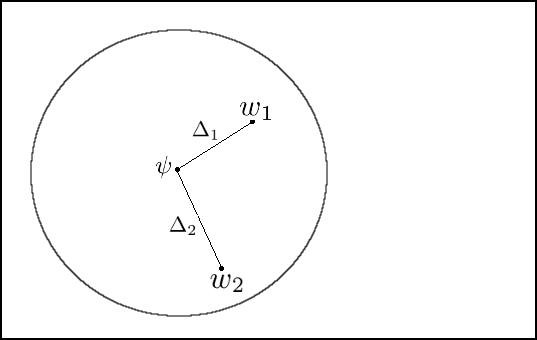
\includegraphics[scale=0.5]{example.png}
	\caption{Rectangle box represents the entire message space. Only one of many balls is shown}
	\label{fig:example}
\end{figure}



The rest of the paper is organised as follows: Section \ref{prelim} discusses the preliminaries needed 
and the ingredients that are used in this paper. Section \ref{sec:imle} explains Interactive MLE scheme
introduced in \cite{imle}, the adversarial model and the security game used. The construction of $\scheme$
is explained in section \ref{sec:constr} and its security is proved in section \ref{sec:res}.
\chapter{Review}
\label{chap:review}

\begin{quote} \small
	We will briefly look at the related works in the Secure Deduplication field
\end{quote}

Douceur et al. \cite{convergentEnc} were the first to propose a novel deterministic cryptosystem
called \textit{convergent encryption} (CE) that enables deduplication to work with
encryption. The idea was to derive the encryption key from the message itself. This
will result in users possessing the same message to end up with the same ciphertext.
\\ \\
Halevi et al. \cite{proofOwner} identified several attacks that exploit client-side
deduplication and introduced the concept of proofs-of-ownership to mitigate these. This
work was extended to get a secure client-side deduplication by Xu et al. in \cite{weakLeakage}.
\\ \\
Bellare et al. in their 2013 paper \cite{mle} formalized the notions of security
in secure deduplication using a new cryptographic primitive called 
\textit{Message-Locked Encryption} (MLE) which subsumes CE. 
The paper was the first to formally argue
the security of secure deduplication and analysed the security of existing schemes as
well as put forward new practical security schemes.
\\ \\
In \cite{imle} Bellare et al. built upon MLE and put forward a new scheme they called
\textit{Interactive Message-Locked Encryption} (iMLE) in which upload and download are
protocols. They modelled privacy and security as games that enabled to argue for stronger notions
of security such as when an adversary controls multiple clients.
\chapter{Preliminaries}
\label{chap:prelims}

\begin{quote} \small
	We discuss in brief the preliminaries that are used in our construction.
\end{quote}

\section{Metric spaces}
A metric space is a set $\msgspc$ along with a distance function $\mathsf{dis}: \msgspc \times \msgspc \rightarrow \RR^+$ such that distances are defined between all members of the set \cite{fuzzy}. In this paper, we will be using the \textit{Hamming metric}.
\subsection{Hamming Metric}
In this metric, $\msgspc = \bin^n$ and $\mathsf{dis}(w,w')$ is the number of positions in which strings $w$ and $w'$ differ.
\\ \\
We now define two functions $\mathsf{Diff}$ and $\mathsf{Comb}$.
\begin{itemize}
	\item[$\mathsf{Diff}$] - It takes as input two $n$-length messages $(w_1, w_2) \in \msgspc \times \msgspc$ and outputs the indices in which $w_1$ and $w_2$ differs. We will refer to this output as $\Delta$, i.e. $\mathsf{Diff}(w_1, w_2) = \Delta$. If the difference between $w_1$ and $w_2$ is bounded by $\tau$, then $|\Delta|$ can be bounded by $O{log(n) \cdot \tau}$.
	\item[$\mathsf{Comb}$] - It takes as inputs, $\Delta$ and a message $w_1 \in \msgspc$ and outputs $w_2 \in \msgspc$ such that $\mathsf{Diff}(w_1, w_2) = \Delta$
\end{itemize}

\section{Error-corecting codes}
We will not be using the traditional definition of codes in this.
We have an $(\msgspc, K, \tau)$ error correcting code. $\msgspc$ is the message space. The code $C$ is a subset of size $K$ of $\msgspc$. The error correcting distance of $C$, denoted by $\tau$, is the largest number $\tau > 0$ such that there is at most one valid code word $c \in C$ for a message $w$ such that $\mathsf{dis}(w,c) \leq \tau$. We denote the encoding and decoding funtions as $\mathsf{Enc}$ and $\mathsf{Dec}$ respectively.
\\ \\The encoding and decoding runs in polynomial time. Let $\mathsf{Dec}$ be the decoding function. We use the term decoding for the map that finds, given $w$, the $c \in C$ such that $\mathsf{dis}(w,c) \leq \tau$\cite{fuzzy} \footnote{For some messages $w$, a corresponding codeword $c$ may not exist, but when it exists it will be unique. We will, for the rest of this paper, assume that decoding always yields a codeword. The scheme can easily be adapted to handle cases when this doesn't happen, taking only a small hit in deduplication level. Decoding is not the inverse of encoding according to this definition. \cite{fuzzy}}.

\section{Randomness Extractors}
We have a family of extractors $\ext = \{\ext_{\secpar}\}$ where $\ext_{\lambda} : \bin^{s(\secpar)} \times \bin^{l(\secpar)} \rightarrow \bin^{\kappa(\secpar)}$. $s$ is the seed length, $l$ is the input length and $\kappa$ is the output length. $\ext_{\lambda}$ is an $(l,m,\kappa,\epsilon)$-strong extractor which means that for all min-entropy  $m$ distributions $W$ on $\bin^l$, $\textbf{SD}((\ext(W; X), X), (U_\kappa,X )) \leq \epsilon $, where $X$ is uniform on $\bin^s$\cite{fuzzy}.

\subsection{MLE}    
The paper \cite{mle} introduced a new cryptographic primitive called MLE that 
enables secure deduplication.
An MLE scheme is a five-tuple of polynomial-time algorithms $\mathsf{MLE}=(\mathcal{P,K,E,D,T})$.
$\mathcal{D}$ and $\mathcal{T}$ are deterministic and the others are randomized.
\begin{displaymath}
\begin{aligned}
\text{Paramter Generation: \ \ \ } & P  \sample \mathcal{P}(1^{\lambda}) \\
\text{Key Generation: \ \ \ } & K  \sample \mathcal{K}_P(M) \\
\text{Encryption: \ \ \ } & C \sample \mathcal{E}_P (K,M) \\
\text{Decryption: \ \ \ } & \mathcal{D}_P (K,C) \in \{0,1\}^* \cup \{ \bot \} \\
\text{Tag Generation: \ \ \ } & T \leftarrow \mathcal{T}_P(C)
\end{aligned}
\end{displaymath}

There is a \textit{message space} associated with every lambda. 
\begin{equation}
\notag
MsgSp_{\mathsf{MLE}}(\lambda) \subseteq \{0,1\}^* \ \ \ \  \forall \lambda \in \mathbb{N}
\end{equation}	

\textit{Decryption Correctness: }
\begin{equation}
\notag
\mathcal{D}_P(K,C) = M\ \ \ \ \  \forall \lambda \in \mathbb{N} , \forall P \in [\mathcal{P}(1^\lambda)]
\end{equation}
\textit{Tag Correctness: } There exists a negligible function $\delta : \mathbb{N} \rightarrow [0,1]$ such that
$\forall \lambda \in \NN$, $P \in [P(\secparam)], \forall M \in$ MsgSp$_\mathsf{MLE}(\lambda)$
\begin{equation}
\notag
Pr[\mathcal{T}_P(C) \neq \mathcal{T}_P(C')] \leq \delta (\lambda)
\end{equation}
where $C \sample \mathcal{E}_P (\mathcal{K}_P(M),M) $ and $C' \sample \mathcal{E}_P (\mathcal{K}_P(M),M $ 
are ciphertexts of the same message.
\\
$\mathsf{MLE}$ is deterministic if $\mathcal{K}$ and $\mathcal{E}$ are deterministic. \\ \\
An MLE scheme exploits the fact that key is generated from the message and therefore people with identical messages will wnd up with identical ciphertexts. A tag is generated from ciphertext. Tags are used to compare different ciphertexts, and tags from different ciphertexts should only match if they are the same. Thus, tags enable comparison for the underlying messages. If a user uploads a ciphertext to a server and the tag of that ciphertext matches the tag of an existing file, then the server can identify that they are the same and thus need not store the redundant copy.

\subsubsection{Privacy for MLE}
Semantic security cannot be achieved using any MLE scheme. If the message space $\msgspc$ is predictable,
the adversary, given an encryption $C$ of $M$, can recover $M$ in $O(|\msgspc|)$ trials.\\
\begin{figure}[H]
	\centering
	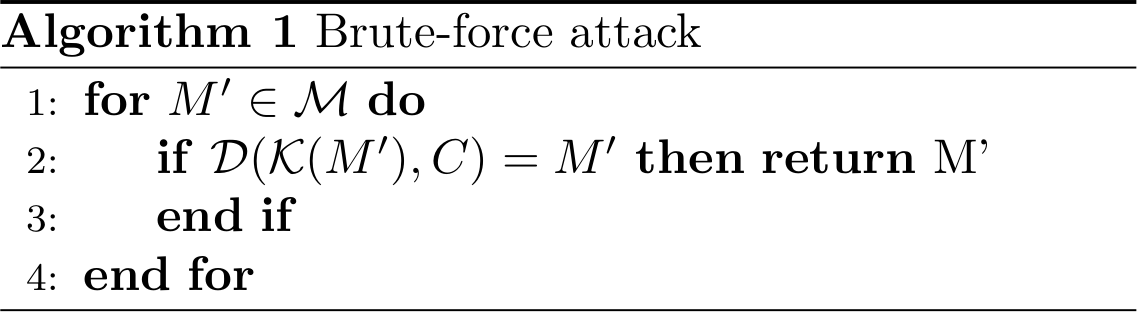
\includegraphics[scale=0.25]{brute}
\end{figure}
So MLE schemes are asked to have semantic security when the message space is unpredictable
\footnote{Unpredictability of message space is formalized later in section \ref{subsec:security}}. 
That is, messages have high min-entropy.

\subsection{Guessing Probability}
The guessing probability of a random variable $X$ is defined using the following equation
\begin{equation}
\textbf{GP}(X) = max_x \prob{X=x} = 2^{-H_\infty(X)}
\end{equation}


\subsection{Hash functions}
A hash function $\mathcal{H}: \bin^n \rightarrow \bin^m$ is a collision-resistant hash function if
\begin{itemize}
	\item $m < n$ and
	\item for all $\ppt \adv$, there exists a negligible function $\negl$ such that for all security parameters $\secpar \in \NN$,
	\begin{equation*}
	\mathsf{Pr} [ ( x_0, x_1) \leftarrow \adv ( \secparam, \mathcal{H} ): 
	x_0 \neq x_1 \wedge \mathcal{H} ( x_0 ) = \mathcal{H}(x_1) ] \leq \negl
	\end{equation*}
\end{itemize}
We denote the family of hash functions to be $\mathsf{H} = ( \mathcal{HK, H} )$

\section{Deterministic Symmetric Encryption}
Deterministic Symmetric Encryption scheme (D-SE), is defined as a pair of algorithms $\mathsf{SE=(E, D)}$. Encryption algorithm $\mathsf{E}$ takes as input the plaintext $m \in \bin^*$ and key $k \in \bin^{\kappa(\secpar)}$ and outputs the ciphertext $c \leftarrow \mathsf{E}(\secparam, k, m)$. Decryption returns the plaintext $m \leftarrow \mathsf{D}(\secparam, k, c)$. \cite{imle} We require D-SE scheme with CPA-security and key-recovery security (KR-secure). We say that a scheme is KR-secure if the probability that the adversary can guess the key from an encryption of a message of his choice is negligible.

\section{Immutability}
A table $T$ is said to be \textit{immutable} if no entry $T[t]$ can be changed once it is set. That is, once the table is initialized, values can only be assigned once \cite{imle}. An immutable table supports the set-iff-empty ($\mathsf{SiffE}$) operation which is defined as below. It takes as input, a table $T$, a message $m$ and an index $f$.

\begin{figure}[H]
	\centering
	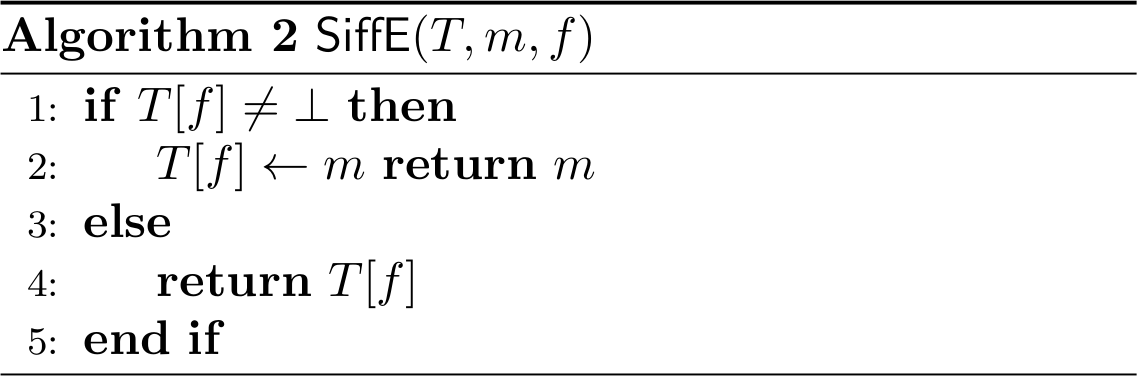
\includegraphics[scale=0.25]{SiffE}
\end{figure}



\chapter{Interactive Message-Locked Encryption}
\label{chap:imle}

\begin{quote} \small
	This chapter looks at the definition and security for interactive message-locked encryption.
\end{quote}

\noindent
In \cite{imle}, MLE was extended to a new scheme called iMLE. An interactive message-locked encryption scheme ($\mathsf{iMLE}$ is defined by four procedures defined below - one algorithm and three protocols.
\begin{enumerate}
	\item $\mathsf{Init}(\secparam)$ - The initialization algorithm run by the server. This will set up the initial server-side state $\serv$.
	
	\item $\mathsf{Reg}$ - This protocol, initiated by the client will register the client with the server. The server returns client parameters $\client \in \bin^*$ which is output by the protocol.
	
	\item $\mathsf{Put}(M, \client)$ - The put protocol takes as input the plaintext and the client credentials. It stores the file and outputs an identifier $f$. Client genertaes key $K \leftarrow \mathcal{K}_{p}(M)$ and then generates the ciphertext $C \leftarrow \mathcal{E}_{p}(K, M)$. Note that $p$ is the public parameter generated by the $\mathsf{Init}$ procedure.
	
	\item $\mathsf{Get}(f, \client)$ - The get protocol takes as input the client parameters and file identifier and outputs the plaintext $m \in \bin^*$
\end{enumerate}

We follow the notation for protocols as given in \cite{imle}.
\begin{itemize}
	\item A protocol $\mathsf{P}$ with 2 players and $q$ rounds is represented using $2 \times q$-tuple of algorithms.
	\item $\mathsf{P}[i,j]$ is the algorithm of the $i^{th}$ player at the $j^{th}$ step where $i \in [2]$ and $j \in [q]$.
	\item $\mathsf{P}[1]$ is the player who starts the protocol. In our case, the client always initiates and hence $\mathsf{P}[1]$ denotes the client.
	\item $\mathsf{P}[2]$ denotes the server.
	\item $1^\lambda$, the input $a$, and a message $M \in \bin^*$ are passed to each algorithm when invoked.
	\item Each algorithm outputs a 3-tuple consisting of output $s'$, an outgoing message $M' \in \bin^*$ and $T$ which is a boolean variable to convey termination.
\end{itemize}

\section{Soundness}
There are two conditions for soundness as described in \cite{imle}
\begin{enumerate}
	\item \textbf{Deduplication: }If a file is uploaded to the server by the client and the file already exists in the server, the storage should not increase by the file size. The increase should be independent of the file and must be bounded. Only a small increase for metadata updation is allowed.\\ Formally, there exists a bound $l: \NN \rightarrow \NN$, such that for all $\serv \in \bin^* $, for all $\client \in \bin^*$, the expected increase in size of $\serv ''$ over $\serv '$ when $(f', \serv ') \sample \mathsf{Put}(\client, m)$ is run and then $(f', \serv '') \sample \mathsf{Put}(\client ', m)$ is run is bounded by $l(\secpar)$ \cite{imle}.
	\item \textbf{Correct recovery of files: }A legitimate client should be able to recover the file at any time after the file has been put on the server. This is formalized by the \textsc{Rec} game (see Figure \ref{fig:REC}). The adversary is given access to procedures \textsc{Reg, Init, Step, Msg, State}.
	\begin{itemize}
		\item \textsc{Reg: }Set up a legitimate client $L$.
		\item \textsc{Init: }Enables adversary $A$ to run protocols on behalf of $L$. $\mathsf{inp}$ and $\mathsf{P}$ are given as inputs to \textsc{Init} where $\mathsf{P} \in \{ \mathsf{Get}, \mathsf{Put} \}$. $\mathsf{inp}$ is a valid input for $\mathsf{P[1,1]}$. Returns $j \in \mathbb{N}$, the instance index to $A$.
		\item \textsc{Step: } Takes as input the instance index $j$ and advances it by one algorithm (or step) if the current instance is still active (not terminated). It returns to $A$ the outgoing message sent. When an instance $j$ terminates, \textsc{WinCheck}is run by \textsc{Step}. \textsc{WinCheck} maintains a table $T$ which stores the message $m$ and identifier $f$ in the $\mathsf{Put}$ protocol. When $j$ is an instance of $\mathsf{Get}$ protocol, \textsc{WinCheck} obtains the identifier $f$ and the recovered message $m'$. This is checked with $T[f]$ to see if it matches. If there is a mismatch, \textsc{WinCheck} sets the $\mathsf{win}$ flag in which case the adversary $A$ wins.
	\end{itemize}
\end{enumerate}

\begin{figure}[H]
	\centering
	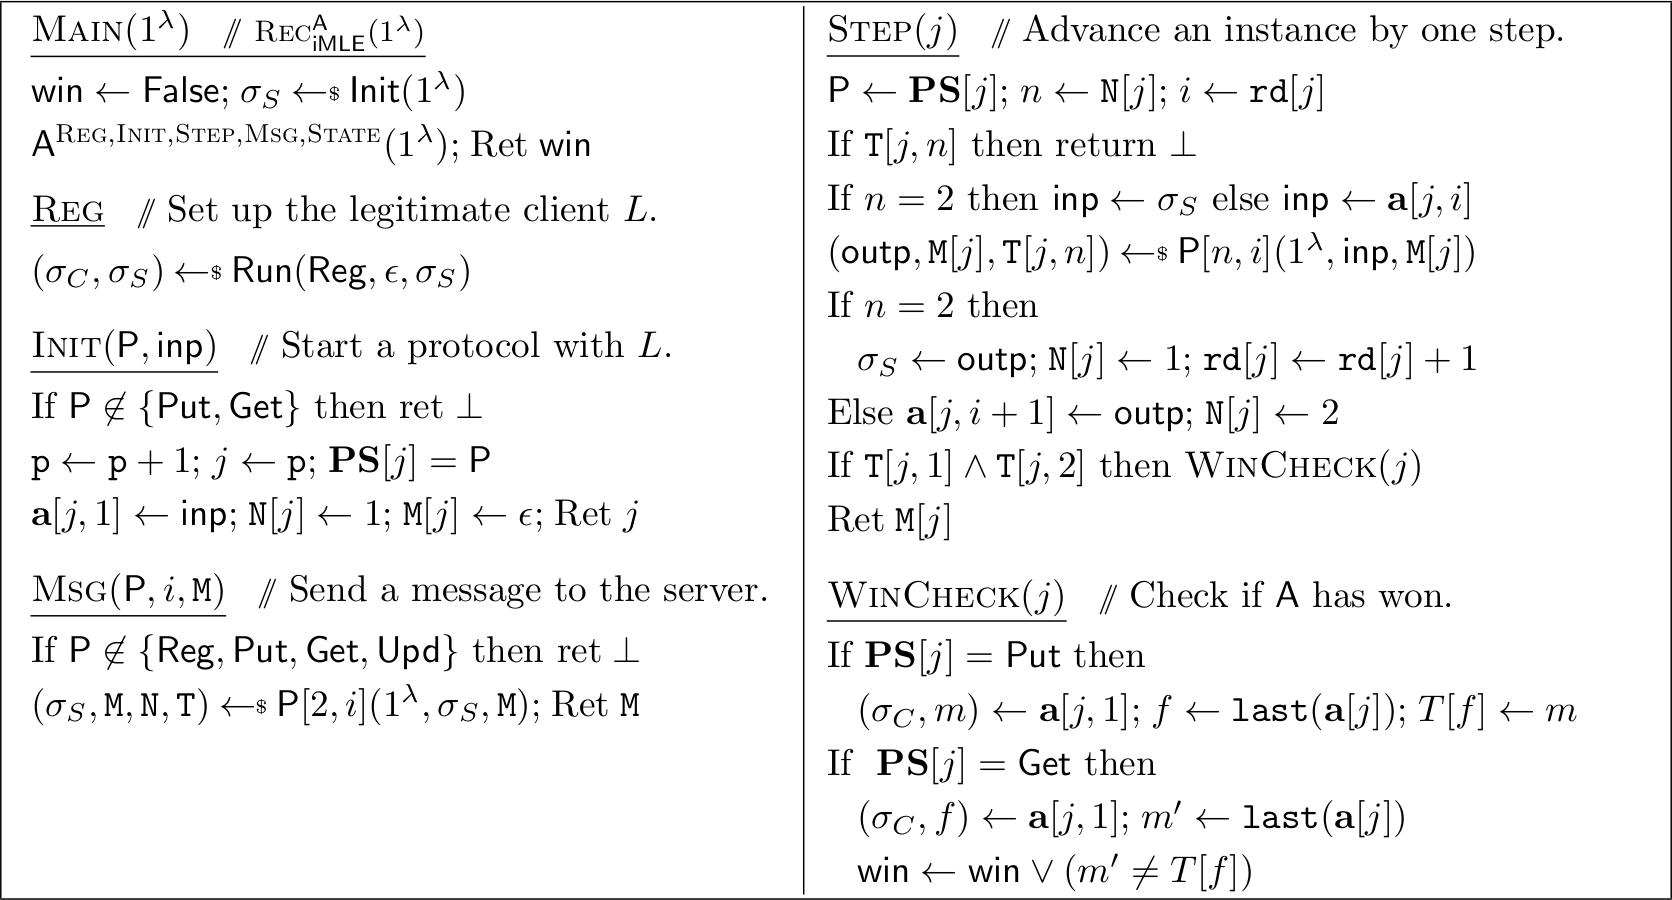
\includegraphics[width=\textwidth]{REC}
	\caption{The recovery correctness game - REC \cite{imle}}
	\label{fig:REC}
\end{figure}

	\section{Security}
	\label{subsec:security}
	The primary requirement for any secure deduplication scheme is security for unpredictable data. If the distribution from which the plaintext comes does not have negligible guessing probabability, then security cannot be achieved.\\ \\
	Privacy for unpredictable messages is captured by the \textsc{Priv} game. Unpredictability is formalized using the following notion of a source.
	\begin{enumerate}
		\item An algorithm called \textit{source} $\mathsf{S}$ which on inputs $\secparam$ and string $d \in \bin^*$ outputs a pair of tuples $(\smzero, \smone)$.
		\item All components of $\smzero$ and $\smone$ are unique. The length of each component is given by function $\ell : \NN \times \NN \rightarrow \NN $. $|\smzero[i]| = |\smone[i]| = \ell(\secpar, i)$. Similarly, there exists $m: \NN \rightarrow \NN $ so that $|\smzero| = |\smone|= m (\secpar)$.
		\item The guessing probability of $\mathsf{S}$ is
		\begin{equation*}
		\textbf{GP}_\mathsf{S}(\secpar) = max_{i,b,d}(\textbf{GP}(\textbf{m}_b[i]))
		\end{equation*}
		when $(\smzero, \smone) \sample \mathsf{S}(\secparam, d)$
		\item To model unpredictability, the guessing probability of the source $\mathsf{S}$ must be negligible.
	\end{enumerate}
	\textsc{Priv} game is formalized as follows.
	\begin{enumerate}
		\item Run \textsc{Init} to set up the server-side state.
		\item Run the source $S$ to get $(\textbf{m}_0, \textbf{m}_1)$. A random bit $b$ is selected and $\textbf{m}_b$ is used as messages to be put in the server.
		\item $A$ is invoked with oracle access to \textsc{Reg, Put, Step, Msg} and \textsc{State}. These oracles behave the same way as in \textsc{Rec} game, except that \textsc{Step} does not call \textsc{WinCheck}. \textsc{Put}($i$) means put plaintext $\textbf{m}_b[i]$.
	\end{enumerate}     
	

\begin{figure}[H]
	\centering
	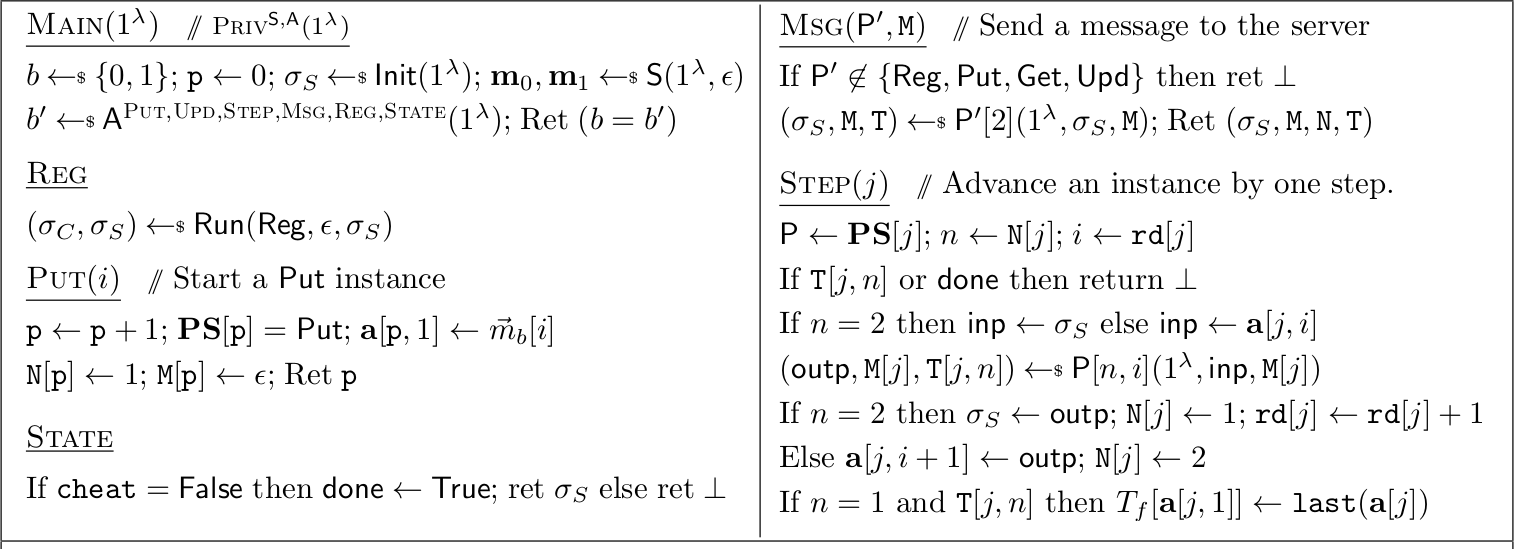
\includegraphics[width=\textwidth]{priv}
	\caption{The privacy game - PRIV \cite{imle}}
\end{figure}

	
	\section{Adversarial Model}
	The adversarial model used in this paper is similar to the one used in \cite{imle}.
	A secure deduplication system consists of a server and several clients. The attacker could control several clients simultaneously and could gain access to server storage. The adversary could also interfere the communications where he can read, relay and drop messages of legitimate clients. To simplify the protocol, we assume that the adversary cannot tamper with message contents, reorder messages within a protocol, or redirect from one protocol to another. The adversarial model captures an iMLE scheme running in the presence of an adversary with above mentioned abilities.
	\\ \\ The adversarial model is achieved by using an abstract game $G$. The games for soundness, security and other properties follow the structure similar to the one below. The objective of the game is for the adversary to violate some property of iMLE guaranteed to legitimate clients. 
	\begin{itemize}
		\item $G$ sets up and controls an instance of a server.
		\item Adversary $\adv$ is invoked with access to a set of procedures.
		\item \textsc{Msg} procedure allows adversary to set up multiple clients and to send arbitrary messages to the server.
		\item \textsc{Init} procedure starts protocol instances on behalf of a legitimate client $L$, using inputs chosen by $A$.
		\item \textsc{Step} procedure advances a  protocol instance by running the next step algorithm.
		\item \textsc{State} procedure returns the server's state - including stored ciphertexts, public parameters, etc. Only read only access is gained using this. Otherwise adversary can always tamper with the ciphertexts and win the game.
	\end{itemize}
\chapter{$ \scheme $ Construction}
\label{chap:constr}

\begin{quote} \small
	We will see the construction of $ \scheme $.
\end{quote}

\section{Construction}

We have with us the following:
\begin{itemize}
	\item A metric space ($\msgspc$, $\mathsf{dis}$)  with hamming distance as the distance metric.
	\item An $(l,m,\kappa,\epsilon)$-strong extractor.
	\item An error-correcting code $C = (\msgspc, K, \tau)$.
	\item A collision resistant hash function family $\mathsf{H}=(\mathcal{HK, H})$.
	\item $\mathsf{SE = (E,D)}$ denotes a symmetric encryption scheme.
\end{itemize}

The $\scheme [C, \mathsf{H}, \mathsf{SE}]$ is defined by one procedure - $\mathsf{Init}$ - and three protocols - $\mathsf{Reg}$, $\mathsf{Put}$ and $\mathsf{Get}$. The server maintains three tables:
\begin{itemize}
	\item $\textbf{fil}$: which contains the encryptions of the files uploaded by the clients. Each ciphertext in this table is indexed using a unique identifier derived from itself which we call the $tag$. This table is immutable.
	\item $\textbf{delt}$: which stores the $\Delta$ as discussed in section \ref{sec:intro}. This table is also immutable.
	\item $\textbf{own}$: which stores the ownership information.
\end{itemize}
\begin{figure}[H]
	\centering
	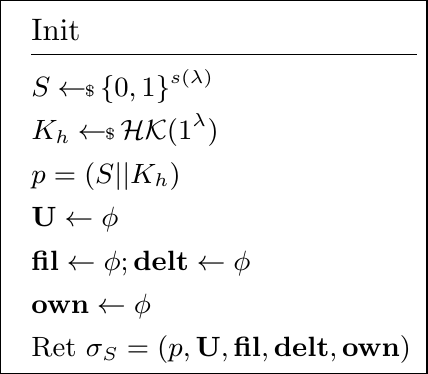
\includegraphics[scale=0.5]{init}    
	\caption{The $\mathsf{Init}$ procedure. This will set up the server, create empty databases $\mathsf{fil}$ and $\mathsf{own}$ and runs $\mathcal{P}(1^{\lambda})$. $\mathsf{fil}$ stores the encrypted files uploaded by the client and is indexed by the tag. $\mathsf{own}$ stores the ownership information and associates with each client, the tag of the files uploaded by the client.}
\end{figure}

\noindent
The $\mathsf{Reg}$ protocol registers a new client with the server. The server picks a unique client identifier and returns it to the client.

\begin{figure}[H]
	\centering
	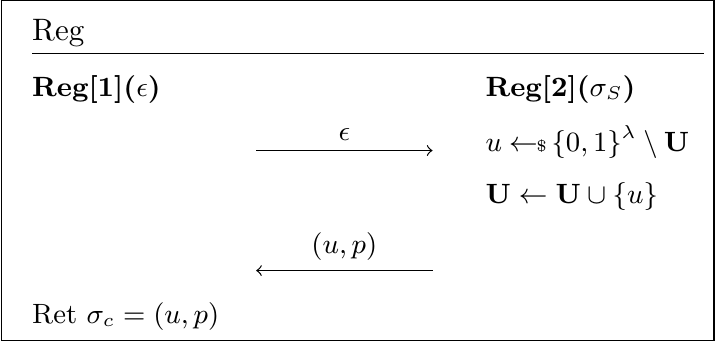
\includegraphics[scale=0.5]{reg}
	\caption{The $\mathsf{Reg}$ protocol. This returns the client parameters $\sigma_c$ which includes the client credentials and the keys generated in \textsc{Init}}	
\end{figure}

\begin{figure}[H]
	\centering
	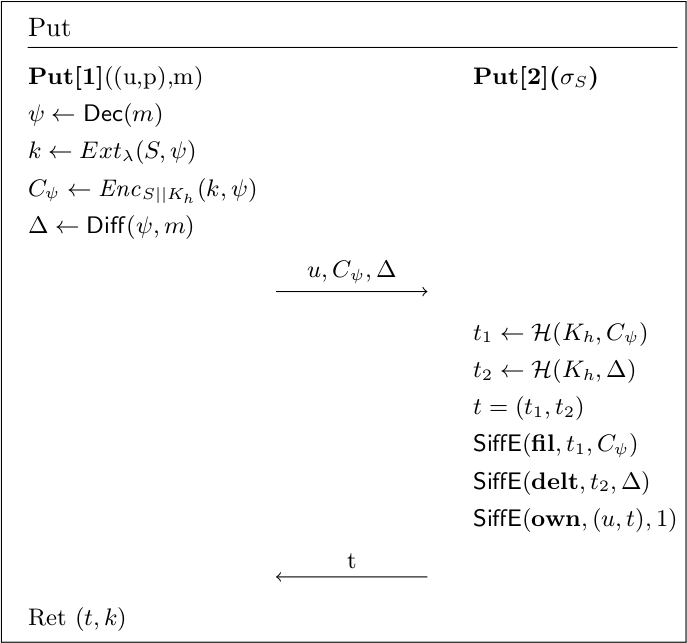
\includegraphics[scale=0.5]{put}
	\caption{The $\mathsf{Put}$ protocol. \textbf{fil}, \textbf{delt} and \textbf{own} tables are immutable. Here the $\Delta$ is stored in $\textbf{delt}$ table and $\textbf{own}$ table stores a $1$ to show that the client with credentials $u$ owns the file with tag $t$}
	\label{fig:put}
\end{figure}

\noindent
In the $\mathsf{Put}$ protocol, the message $m$ is first mapped to its codeword $\psi$. $\Delta = \mathsf{Diff}(\psi, m)$ is computed. The client then sends $(\mathsf{E}(k,\psi), \Delta)$ to the server. The server hashes $\psi$ and $\Delta$ to get the tag $t = (t_1 = \mathcal{H}(K_h, \psi), t_2 = \mathcal{H}(K_h, \Delta))$. The message is finally stored in the $\textbf{fil}$ and $\textbf{delt}$ tables. $\textbf{fil}[t_1] = C_\psi$ and $\textbf{delt}[t_2] = \Delta$. The ownership table is also updated to reflect this. $\textbf{own}[u,t]=1$. If another client (with credentials $u'$) tries to upload the same file $m$, then the server only needs to update it on the ownership table. $\textbf{own}[u',t]=1$.

\begin{figure}[H]
	\centering
	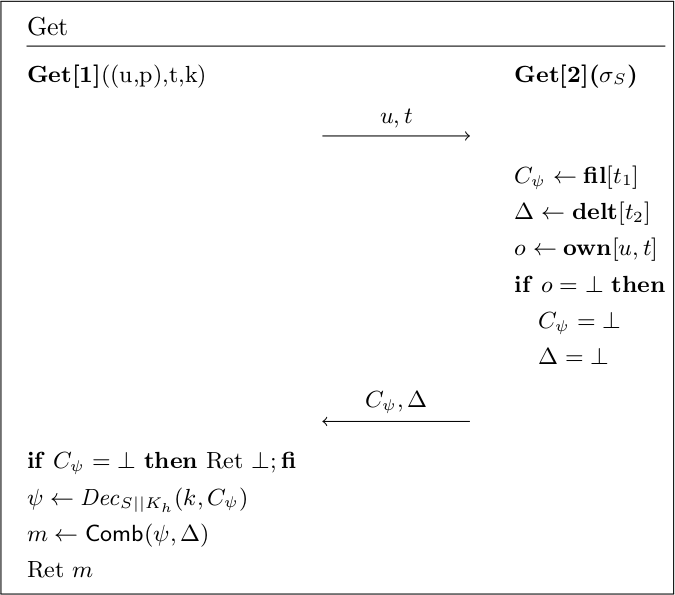
\includegraphics[scale=0.5]{get}
	\caption{The $\mathsf{Get}$ protocol.}
	\label{fig:get}
\end{figure}

\noindent
In the $\mathsf{Get}$ protocol, client sends the tag $t$ and credentials to the server. The server verifies if the client owns the file  by checking the ownership table and if it does, returns $C_\psi$ and $\Delta$. The client decrypts $C_psi$ to get $\psi$ and applies $\mathsf{Comb}(\psi, \Delta)$ to get back $m$.

\chapter{Results}
\label{chap:results}

\section{Deduplication}
It is clear that $\scheme$ enables deduplication since different users with the same file will end up with the same tag and therefore only one copy is saved in the server. We will now state two theorems regarding the privacy and security of $\scheme$ 

\section{Recovery}
\begin{theorem}
	If $\mathcal{E}$ is a correct deterministic symmetric encryption (D-SE) and $\mathsf{H}$ is collision resistant, then the above scheme $\scheme [\mathsf{H},\mathcal{E}, C]$ is \textsc{Rec}-secure.
\end{theorem}
\subsubsection*{Proof}
For adversary $A$ to win the \textsc{Rec} game, there must be a mismatch in the plaintext $m$ put on the server and the plaintext $m'$ recovered using $\mathsf{Get}$.\\ 
Whenever the client sends the ciphertext $C=(C_\psi, \Delta)$, the tag $t=(t_1, t_2)$ is computed by the server and \textbf{fil}[$t_1$], \textbf{delt}[$t_2$] and \textbf{own}[$t$] are filled. Since the tables are immutable, the ciphertext will not change once it is entered. When the client requests for tag $t$, the server checks \textbf{own}[$t$] and returns \textbf{fil}[$t_1$] and \textbf{delt}[$t_2$]. Thus recovery correctness is always ensured except when a collision occurs. Since we are using a collision resistant hash function, the probability of this happening is negligible.

\section{Privacy}
\begin{definition}
	The error-correcting code $C=(\msgspc, K, \tau)$ is said to be compatible with a source $\mathsf{S}$ with min-entropy $\mu(\secpar)$ iff $2^{\mu(\secpar)-\tau}$ is negligible.
	\label{def}
\end{definition}
This definition is used to put a constraint on the error correcting distance of $C$. If the error correcting distance $\tau$ is large, we cannot ensure privacy. This is because we are leaking $\Delta$ which has an entropy bounded by $\tau$. Thus even after leaking $\tau$ bits of information, there needs to be enough entropy in the message space to ensure unpredictability.

\begin{theorem}
	If $\mathcal{E}$ is CPA-secure and KR-secure and the code $C=(\msgspc, K, \tau)$ is compatible with the source $S$, then $\scheme_{RO}$[$\mathcal{E}$, $C$] \footnote{$\scheme_{RO}$ is the ROM analogue of $\scheme$ which models $\mathsf{H}$ as a random oracle} is \textsc{Priv}-secure.
\end{theorem}

\subsubsection*{Proof}
In the \textsc{Priv} game, the source $S$ outputs two vectors $\textbf{m}_0, \textbf{m}_1$ where $\textbf{m}_i$ is a vector over $\bin^*$. A random bit $b$ is chosen. Adversary can put and get components of $\textbf{m}_b$ and finally learns the server-side state. $A$ wins if it correctly guesses b.\\

Let $\mathsf{S}$ be an unpredictable PT source and $C$ be a compatible error correcting coding scheme. $\mathsf{S}$ outputs $m(\secpar)$ plaintexts each of length $\ell(\secpar, i)$. We denote the polynomial time adversary using $A$. The number of messages stored by the adversary is bounded by $n: \NN \rightarrow \NN$ and the number of random oracle queries made by source and adversary is bounded by $q_S(\secpar): \NN \rightarrow \NN $ and $q_A(\secpar): \NN \rightarrow \NN $
\\ 
We will use a hybrid argument to show the privacy of the $\scheme$. Consider the \textsc{Priv} game in the figure \ref{fig:priv}.\\
\begin{figure}
	\centering
	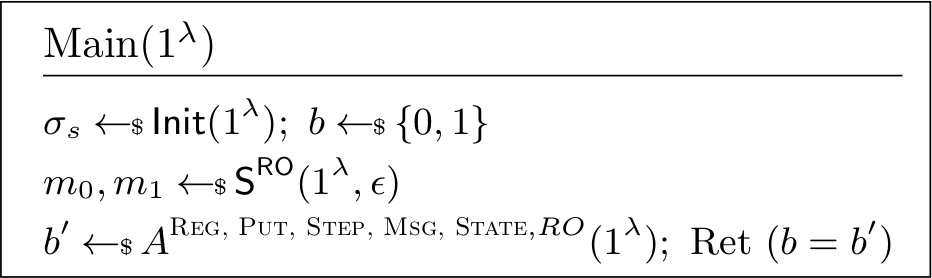
\includegraphics[scale=0.3]{Priv_game}
	\caption{The \textit{main} function of the \textsc{Priv} game}
	\label{fig:priv}
\end{figure}

\begin{figure}
	\centering
	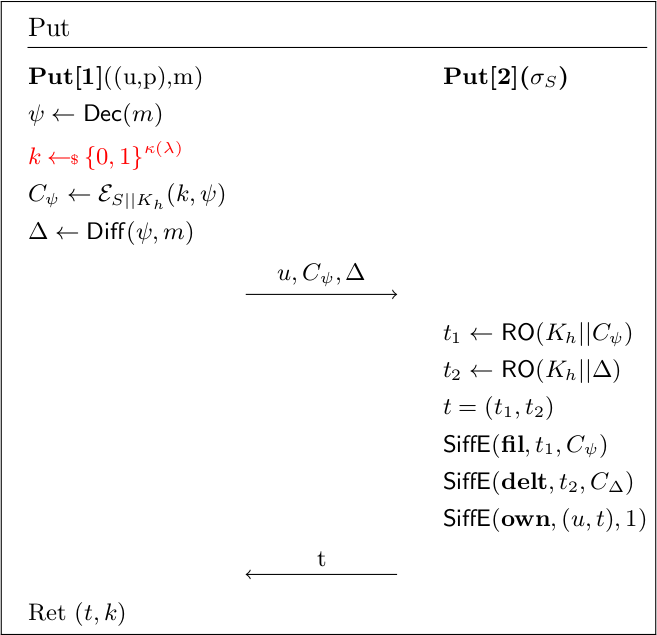
\includegraphics[scale=0.4]{H2}
	\caption{The $\mathsf{Put}$ protocol in game $H_2$}
\end{figure}

\begin{figure}
	\centering
	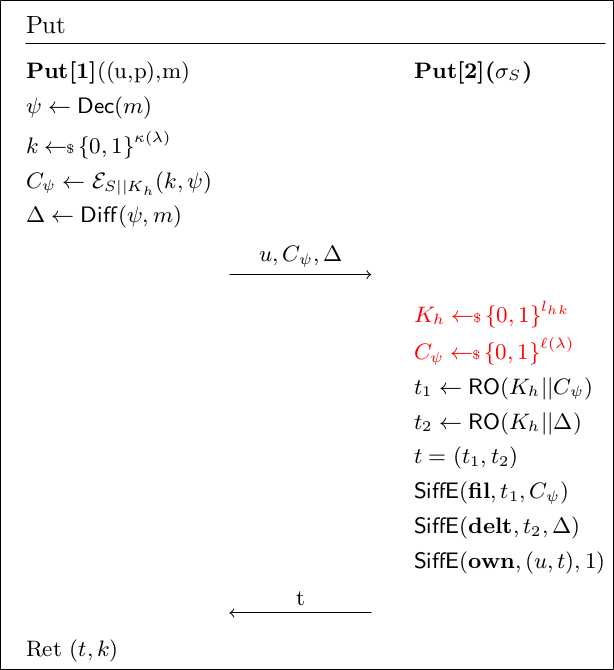
\includegraphics[scale=0.4]{H3}
	\caption{The $\mathsf{Put}$ protocol in game $H_3$}
\end{figure}

\noindent
The \textsc{Reg, Step, Msg} and \textsc{State} are same as in the \textsc{Priv} game. The $\mathsf{Put}$ protocol changes in each hybrid game.
Let $H_1$ denote the actual $\mathsf{Put}$ protocol from figure \ref{fig:put} with the only difference being that instead of $H$, it uses $RO$. In the game $H_2$, the $k$ is sampled randomly instead of using the extractor output. This will give the adversary with an $\epsilon$ advantage since the extractor output is $\epsilon$ close to uniform distribution.

\begin{equation}
\prob{\textsc{Priv}_\scheme^{\mathsf{S,A}}(a^\lambda)} = \prob{H_1^{\mathsf{S,A}}} \leq \prob{H_2^{\mathsf{S,A}}} + \epsilon
\end{equation}

In $H_3$, the RO queries for $t_1$ are made using random strings. The adversary can detect this only if it had queried $\mathsf{RO}(K_h||C_\psi)$. The probability for this bad event is bounded by $q_A(\lambda)n(\lambda)/2^{\ell(\secpar, i) - \tau}$ where $q_A$ is the bound on the number of RO queries made by $A$.

\begin{equation}
\prob{H_2^{S,A} \text{ sets }\mathsf{bad}} -
\prob{H_3^{S,A} \text{ sets }\mathsf{bad}}  \leq \frac{q_A(\lambda)n(\lambda)}{2^{m(\secpar) - \tau}}  + q_s(\lambda)n(\lambda)GP_S(\lambda)
\end{equation}

In game $H_4$, $\psi$ is an encryption of a random string. The CPA-security of the $\mathit{Enc}$ means that adversary cannot distinguish with any significant advantage. In game $H_4$, there is no information about the message $m$ at all other than $\Delta$. By Definition \ref{def}, the min-entropy of the message $m$ is still high. Thus,

\begin{equation}
\prob{H_4^{A} \text{ sets }\mathsf{bad}} \leq  \frac{q_A(\lambda)n(\lambda)}{2^{m(\secpar) - \tau}} + q_s(\lambda)n(\lambda)GP_S(\lambda)
\end{equation}

\begin{figure}[H]
	\centering
	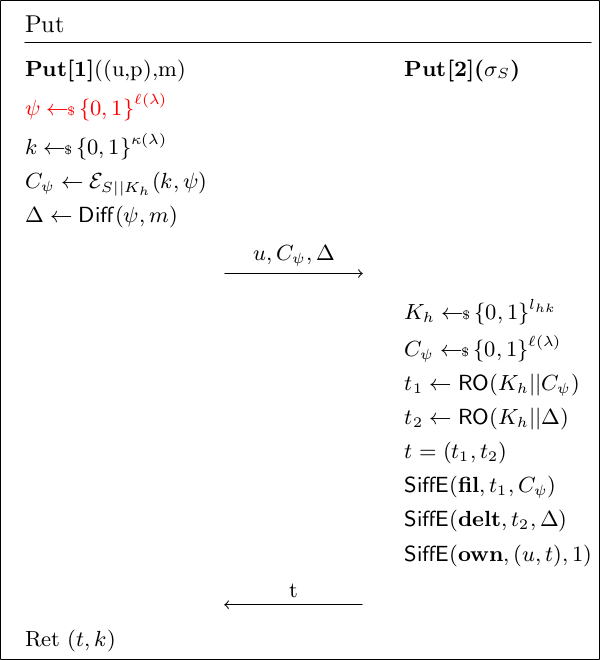
\includegraphics[scale=0.5]{H4}
	\caption{The $\mathsf{Put}$ protocol in game $H_4$}
\end{figure}        

Since at each of the hybrid steps there is only a negligible hit in the probability of adversary winning, adding all the probabilities will still give only a negligible advantage to the adversary. Thus $\scheme$ is \textsc{Priv}-secure.\\ \\
The scheme is efficient since when files that are close together are uploaded, the storage grows only by an additional factor of $\Delta$ for each new file. If the files are identical, then the overhead is minimal.
\chapter{Conclusion and Future Works}
\label{chap:future}

We have put forward a scheme called $\scheme$ that enables deduplication across files and have proved its soundness and privacy. We are able to save space by only storing the ``delta" between two files that are close to each other and maps to the same codeword.



% \backmatter % book mode only
% \appendix
% \include{Appendix1/appendix1}
% \include{Appendix2/appendix2}

\bibliographystyle{plainnat}
%\bibliographystyle{Classes/CUEDbiblio}
%\bibliographystyle{Classes/jmb}
%\bibliographystyle{Classes/jmb} % bibliography style
% \renewcommand{\bibname}{References} % changes default name Bibliography to References
% \bibliography{References/references} % References file
\bibliography{references}
\end{document}
